% Based on the IEEE Journal style.
\documentclass[10pt,a4paper,compsoc]{IEEEtran}

\usepackage{graphicx}
\usepackage[cmex10]{amsmath}
% TODO: Deutsche oder Englische Sprache wählen
\usepackage[ngerman]{babel} % Deutsche Ausarbeitung
% \usepackage[USenglish]{babel} % Englische Ausarbeitung
\usepackage{url}
\usepackage{hyperref}
\usepackage{breakurl}
\usepackage[T1]{fontenc}
\usepackage[utf8]{inputenc}
% TODO: \usepackage{ccicons} bietet wesentlich hübschere Icons, ist aber nicht auf jedem System verfügbar. Für ccicons muss weiter unten \cc\bysa in \ccbysa geändert werden.
\usepackage{cclicenses}

\usepackage{tabularx}
\usepackage{booktabs}
\usepackage{caption} 
\captionsetup[table]{skip=10pt}

\begin{document}

% TODO: Titel, Autor und E-Mail Adresse anpassen
\title{OpenShift}
\author{%
\IEEEauthorblockN{Thomas Witte}\\
\IEEEauthorblockA{\url{thomas.witte@uni-ulm.de}}%
}

% TODO: Bitte hier Titel des Seminnars und Semester anpassen
\markboth{Ausgewählte Themen verteilter Systeme, SS 2013, Institut für Verteilte Systeme, Universität Ulm}{}
% English: \markboth{Seminar title, WS/SS 20XX, Institut of Distributed Systems, University of Ulm}{}

% TODO: Creative Commons Lizenz: bitte auskommentieren, falls nicht gewünscht
\IEEEpubid{\sf%
\cc\bysa
\quad
Diese Arbeit ist lizensiert unter einer Creative Commons Namensnennung - Weitergabe unter gleichen Bedingungen 3.0 Deutschland Lizenz.}
% English:
% \IEEEpubid{\sf%
% \ccbysa
% \quad
% This work is licensed under a Creative Commons Attribution-ShareAlike 3.0 Germany License.}

\maketitle

\begin{abstract}
Cloud Computing und im speziellen Platform as a Service Dienste ermöglichen kostengünstig und energieeffizient Webanwendungen zu hosten und somit für kleine Unternehmen finanzielle Risiken durch die Anschaffung von Hardware zu minimieren. Die Arbeit beschäftigt sich mit OpenShift, einer seit 2011 entwickelten, quelloffenen PaaS Plattform und bietet einen Überblick über den Aufbau einer OpenShift Anwendung, die Verzeichnisstruktur, Deploymentmechanismen und Möglichkeiten der Skalierung. Im zweiten Teil wird die zu Grunde liegende Architektur, Redundanzaspekte und die logische Unterteilung in Nodes und Broker sowie die Kommunikation zwischen diesen Teilen näher betrachtet.
\end{abstract}

\section{Einführung}

% TODO: \IEEEPARstart wird nur am Anfang des ersten Absatzes im Paper verwendet, *nicht* am Anfang jeder Section.
\IEEEPARstart{D}er Begriff Cloud Computing ist sehr weit gefasst und wird derzeit für fast jeden Internetdienst oder netzwerkbasierten Service genutzt. Eine deutlich bessere wenn auch oft nicht eindeutige Einordnung dieser Dienste bieten die Begriffe „Software as a Service“ (SaaS), „Platform as a Service“ (PaaS) und „Infrastructure as a Service“ (IaaS) \cite{nist_cc}. Der Dienst wird dabei durch die Ebene im Hardware-/Software-Stack charakterisiert auf der der Kunde ihn nutzen kann.
Abbildung~\ref{fig:cloudcomputing} verdeutlicht diese vertikale Unterteilung und liefert Beispiele für Dienste die in die jeweilige Kategorie fallen.
\begin{figure}[htbp]
	\centering
	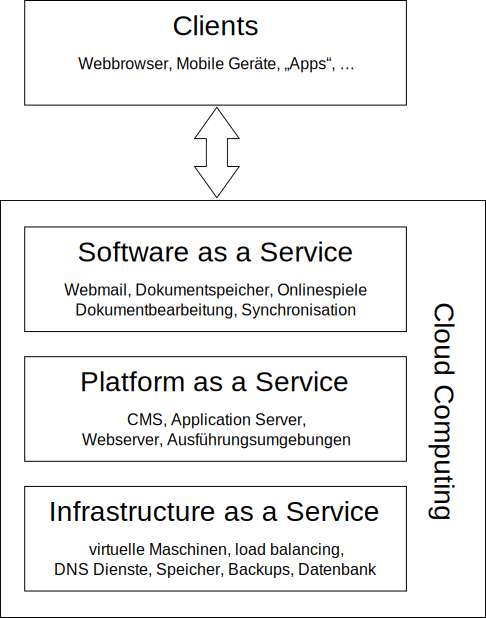
\includegraphics[width=0.9\linewidth]{imgs/cloudcomputing}
	\caption{Kategorisierung verschiedener Cloud Computing Dienste.}
	\label{fig:cloudcomputing}
	% Bildquelle Wikipedia cloud computing
\end{figure}
Diese Arbeit betrachtet Cloud Computing fast ausschließlich auf der PaaS Ebene und bietet einen Einblick in den OpenShift PaaS Dienst sowie die zu Grunde liegende Technologie.

PaaS-Dienste wie OpenShift empfehlen sich gerade für kleinere Firmen und Internetplattformen, deren Geschäftsmodell und Erfolgsaussichten noch nicht feststehen. Dank des einfachen Deployments können die Entwickler schnell eine erste Version der Seite verfügbar machen, ohne durch die Beschaffung von Hardware oder langfristige Mietverträge für Server in Rechenzentren finanzielle Risiken tragen zu müssen. Solange die Seite wenig bekannt und besucht ist werden keine Kosten dafür fällig; nimmt die Popularität schnell zu können schnell und automatisiert weitere Ressourcen verfügbar gemacht werden.

In Abschnitt~\ref{sec:related} werden zu OpenShift ähnliche, konkurrierende Dienste aufgelistet. Es folgt ein Blick auf die Funktionen von OpenShift in Abschnitt~\ref{sec:user} sowie auf einige OpenShift Interna in Abschnitt~\ref{sec:tech}. Eine kurze Zusammenfassung liefert schließlich Abschnitt~\ref{sec:sum}.

\subsection{Geschichte von OpenShift}
Im November 2010 übernahm RedHat den kalifornischen Cloudspezialisten Makara. Dessen Deployment- und Managementlösungen wurden in Verbindung mit RedHat eigenen Technologien zur Plattform OpenShift vorangetrieben \cite{openshift_primer}. Nach der offiziellen Ankündigung im Mai 2011 wurden kostenlose Zugänge zur Developer Preview angeboten; seit November 2012 existiert die finale, auf OpenShift Origin beruhende Version \cite{os_enterprise}.

OpenShift war und ist dabei immer wieder größeren Änderungen unterzogen: so wurde die ursprüngliche Dreiteilung in OpenShift Express, OpenShift Flex und OpenShift Power aufgegeben und es werden mittlerweile nur noch OpenShift Online zur privaten und kommerziellen Nutzung in der RedHat Cloud sowie OpenShift Enterprise zur Nutzung der OpenShift Technologie in eigenen Rechenzentren durch RedHat angeboten \cite{cloud_kueche}.

\subsection{OpenShift Origin}
Als OpenShift Origin wurde der Quellcode der Plattform OpenShift sowie zugehöriger Clienttools unter der Apache 2.0 Lizenz freigeben \cite{os_code}\cite{apache_lic}, sodass nicht nur eine in geringem Umfang kostenlose Nutzung von OpenShift auf den Servern von RedHat möglich ist, sondern auch das Aufsetzen, Nutzen und Weiterentwickeln der Plattform unabhängig von RedHat.

\section{Übersicht anderer PaaS Anbieter}
\label{sec:related}
Neben OpenShift existieren eine vielzahl weiterer PaaS Angebote, die teilweise einen sehr ähnlichen Fokus, teilweise aber auch andere Schwerpunkte besitzen.

Zu den wichtigsten Alleinstellungsmerkmalen von OpenShift gegenüber konkurrierenden Produkten wie AWS Elastic Beanstalk von Amazon \cite{aws}, Microsofts Azure Cloud \cite{azure} und Googles App Engine \cite{app_engine} zählen die quelloffene Plattform sowie das Ausführen beliebigen Codes, solange dieser unter Red Hat Enterprise Linux (RHEL) lauffähig ist und geltende SELinux Richtlinien nicht verletzt. Dadurch können statt aus einer begrenzten Anzahl angebotener Plattformen und Programmiersprachen zu wählen fast beliebige genutzt werden \cite{os_paas}. Zu beachten ist dabei jedoch, dass sich die in Abschnitt~\ref{sec:scale} angesprochenen Möglichkeiten zur automatischen Skalierung über mehrere Instanzen beziehungsweise Ausführungseinheiten (hier „Gears“ genannt) auf Anwendungen beschränken, die einen der mitgelieferten, bereits vorkonfigurierten Anwendungsserver („Cartridge“) nutzen.

AWS Elastic Beanstalk wurde als Erweiterung der IaaS-Dienste Amazons konzipiert und nutzt daher direkt Amazon EC2, Elastic Load Balancing, Auto Scaling und S3 Storage. Zur Nutzung des PaaS Dienstes fallen keine weiteren Kosten außer für die Nutzung der zu Grunde liegenden Infrastruktur an. Als Anwendungsserver werden nur Apache (PHP, Python), Passenger (Ruby), Tomcat (Java) und IIS (.NET) unterstützt.

Microsoft bietet mit Azure Cloud wie Amazon sowohl PaaS als auch IaaS Dienste. Der PaaS Dienst unterstützt dabei offiziell Python, Java, node.js, .NET und PHP; weitere Sprachen werden durch die Community unterstützt. Zur Speicherung persistenter Daten steht SQL Azure zur Verfügung.

Die geringste Flexibilität bietet Googles App Engine, die nur Java oder Python als Sprache ermöglicht. Auf die Konfiguration des Anwendungsservers oder der Datenbank besteht dabei kein direkter Einfluss; die Kommunikation erfolgt rein mittels Standards wie der Servlet-API oder der JPA.

OpenShift ist zusätzlich der einzige der genannten Services, dessen Software vollständig quelloffen ist, sodass kein „Vendor-Lock-in“ besteht und gehostete Anwendungen ohne Anpassungen auf eigene Server oder zu anderen Anbietern migriert werden können.

\section{OpenShift aus Nutzersicht}
\label{sec:user}
Im folgenden wird OpenShift aus der Sicht eines Benutzers geschildert. Benutzer ist in diesem Fall der Programmierer oder Betreiber eines Internetdienstes, dessen Ziel es ist, möglichst einfach und schnell seine Anwendung im Internet verfügbar zu machen oder zu testen. PaaS-Dienste bieten hierbei vielerlei Vorteile:
Es entstehen keine Kosten für die Anschaffung von Serverhardware. Auch die Betriebskosten bleiben bei geringer Bekanntheit oder Nutzung der Anwendung gering.
Ändert sich die Last durch steigende Bekanntheit oder nachlassendes Interesse lässt sich die verfügbare Rechenleistung sehr schnell erhöhen oder senken.
Die Entwickler werden entlastet, da der Aufwand für Konfiguration und Pflege des gesamten restlichen Soft- und Hardwarestacks entfällt.
Durch Lastverteilung und höhere Auslastung der Server kann zudem Energie gespart werden.

Aus diesem Grund gehen die folgenden Abschnitte auf mögliche Plattform/Sprachkombinationen, nötige Schritte zur Vorbereitung der eigenen Anwendung für OpenShift sowie deren Deployment ein. 

\subsection{Mögliche Plattformen/Cartridges}
Eine Anwendung in OpenShift beinhaltet neben dem Code des Nutzers ein oder mehrere vorkonfigurierte Softwarepakete, sogenannte Cartridges. Hierbei stehen einige, hier näher vorgestellte, Cartridges als Teil von OpenShift Origin immer zur Verfügung; speziellere Plattformen oder Software können entweder in Form von Community-Cartridges, oder selbst durch „Do It Yourself“-Cartridges bereitgestellt werden \cite{os_cartridge}.

Die offiziell bereitgestellten Cartridges lassen sich in zwei Kategorien einteilen:

\paragraph*{Web-Cartridges}
Hierunter fallen Ausführungsumgebungen wie PHP, Python, ruby, node.js oder Perl, sowie Server wie Tomcat, JBoss AS oder Zend. Alternativ kann auch eine leere Anwendung mittels der DIY-Cartridge („Do-It-Yourself“) erstellt werden.

\paragraph*{Addon-Cartridges} Dies sind Datenbanken wie MySQL, MongoDB oder PostgreSQL sowie weitere Komponenten wie ein Cron-Dienst, Monitoring-Dienste oder Managementprogramme wie phpMyAdmin.

\begin{figure}[htbp]
\centering
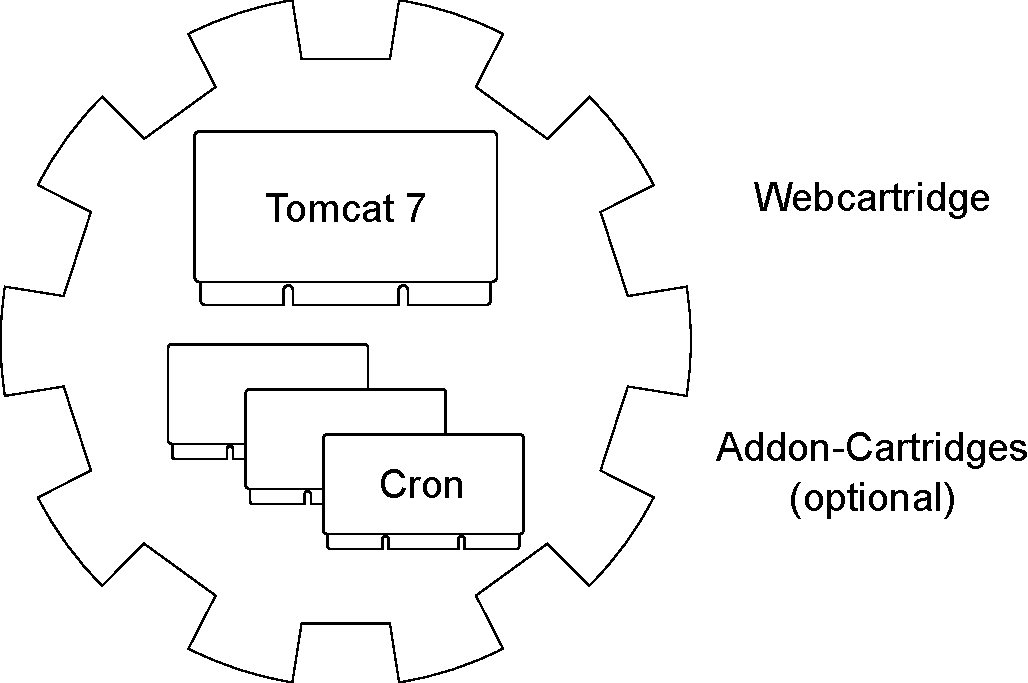
\includegraphics[width=0.8\linewidth]{imgs/cartridges}
\caption{Aufbau einer nicht skalierenden, auf Tomcat basierenden Anwendung.}
\label{fig:cartridges}
\end{figure}

Jede Anwendung muss dabei genau eine Web-Cartridge nutzen. Diese muss beim Erstellen der Anwendung angegeben weden und lässt sich nicht ändern. Addon-Cartridges können in beliebiger Kombination sofort oder zur Laufzeit hinzugefügt oder entfernt werden \cite[S. 28]{os_user_guide}.

\subsection{Vorbereitung der eigenen Anwendung}
Die Anpassung einer eigenen Anwendung zur Nutzung von OpenShift erfolgt in wenigen Schritten.

Zuerst müssen Dateipfade im Code so angepasst werden, dass Dateien im persistenten Speicher gespeichert werden. Jedem Gear steht dabei ein Gigabyte persistenter Speicher zur Verfügung \cite[S. 14]{os_user_guide}, der entsprechende Verzeichnispfad wird als Umgebungsvariable \verb!OPENSHIFT_DATA_DIR! bereitgestellt. Werden Dateien außerhalb dieses Verzeichnisses gespeichert, gehen diese spätestens bei einer Migration auf einen anderen Node oder dem zwischenzeitlichen Deaktivieren der Anwendung verloren. Eine grobe Übersicht über die Verzeichnisstruktur einer OpenShift-Instanz wird in Abbildung~\ref{fig:directories} gezeigt.
\begin{figure}[htbp]
\centering
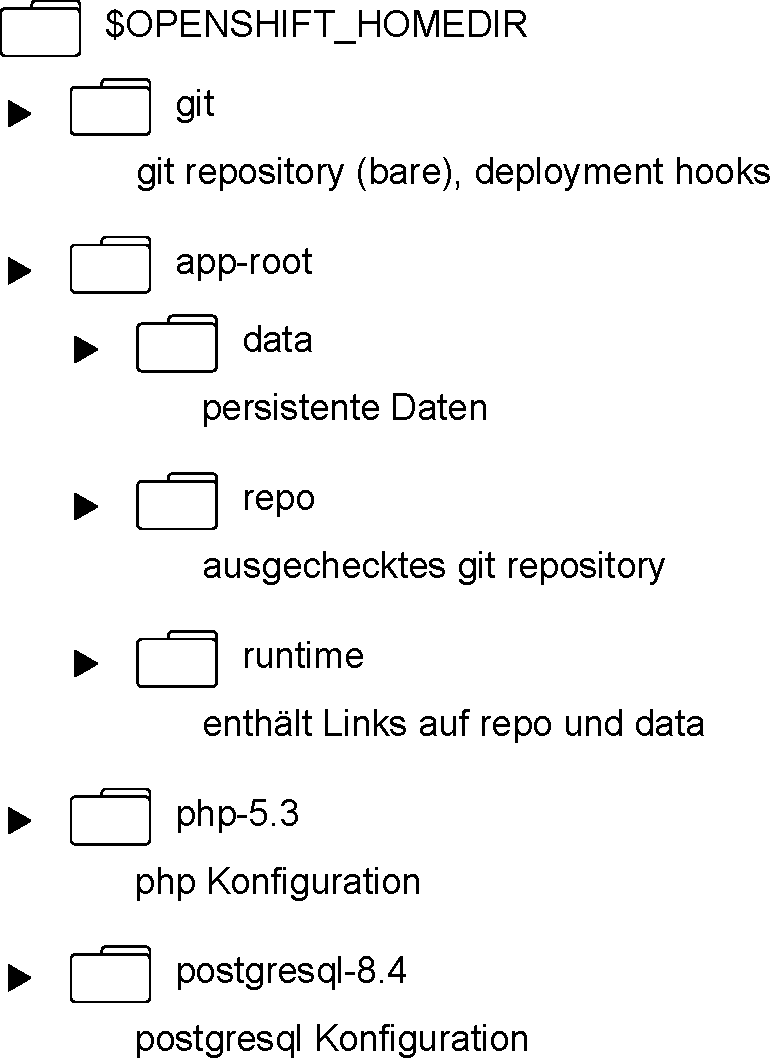
\includegraphics[width=0.7\linewidth]{imgs/directories}
\caption{Beispielhafte Verzeichnisstruktur eines OpenShift Gears mit installierten PHP und PostgreSQL Cartridges \cite{os_architecture}.}
\label{fig:directories}
\end{figure}

Weitere Umgebungsvariablen enthalten Pfade zu Log-Verzeichnissen, Datenbankzugangsdaten, etc.; eine Übersicht der wichtigsten Variablen liefert Tabelle~\ref{tab:variables}.
\begin{table}[htbp]
\centering
\begin{tabularx}{\columnwidth}{XX}
\toprule
Umgebungsvariable & Beschreibung \\
\midrule
OPENSHIFT\_HOMEDIR & Basisverzeichnis der OpenShift Anwendung \\
OPENSHIFT\_DATA\_DIR & Verzeichnis in dem persistente Daten gespeichert werden können \\
OPENSHIFT\_TMP\_DIR & Verzeichnis für temporäre Dateien \\
OPENSHIFT\_REPO\_DIR & Verzeichnis, in das die Anwendung deployed wurde \\
OPENSHIFT\_X\_LOG\_DIR & Logverzeichnis der Cartridge X\\
OPENSHIFT\_X\_DB\_LOG\_DIR & Logverzeichnis der Datenbank X\\
\midrule
OPENSHIFT\_APP\_DNS & DNS-Adresse der Anwendung \\
OPENSHIFT\_APP\_NAME & Name der Anwendung \\
OPENSHIFT\_INTERNAL\_IP & IP-Adresse der Anwendung \\
OPENSHIFT\_INTERNAL\_PORT & Port auf dem die Anwendung lauscht \\
\midrule
OPENSHIFT\_X\_DB\_HOST & Host auf dem Datenbank X läuft \\
OPENSHIFT\_X\_DB\_PORT & Port für Verbindungen zu Datenbank X \\
OPENSHIFT\_X\_DB\_USERNAME & Benutzername für den Datenbankzugriff \\
OPENSHIFT\_X\_DB\_PASSWORD & Passwort um auf die Datenbank zuzugreifen \\
\bottomrule
\end{tabularx}
\caption{Übersicht wichtiger durch OpenShift gesetzter Umgebungsvariablen \cite[S. 59]{os_user_guide}.}
\label{tab:variables}
\end{table}

Alle Verzeichnispfade außer \verb!OPENSHIFT_TMP_DIR! sind relative Pfade bezüglich \verb!OPENSHIFT_HOMEDIR!.

Möglicherweise notwendige Konfigurationsänderungen der Cartridges beziehungsweise der Import eines Datenbankschemas kann entweder manuell durch ssh-Zugriff auf die Anwendungsinstanz geschehen oder automatisiert durch entsprechende Deployment-Hooks, die zum Beispiel bei jeder Aktualisierung der Anwendung ausgeführt werden. Diese Hooks werden im nächsten Abschnitt näher erläutert.

%https://www.openshift.com/page/openshift-environment-variables

%Umgebungsvariablen zum Datenbankzugang, allgemeine Verzeichnisstruktur
%persistenter Speicher

\subsection{Deployment}
Das Deployment, also das Kopieren und Starten der Anwendung auf dem Server, erfolgt unter OpenShift mittels git \cite{git}. Dies vereinfacht die Integration in den Workflow der Entwicklung, ermöglicht eine Versionierung und Versionsverwaltung der ausgelieferten Anwendung und erspart die Einarbeitung in spezielle Deploymentwerkzeuge.

Beim Erstellen einer Anwendung wird automatisch ein git-Repository gleichen Namens angelegt und das git-Verzeichnis innerhalb des Gears in dem die Anwendung läuft als remote hinzugefügt. Die deployte Anwendung wird aus diesem git-Verzeichnis immer dann gepullt wenn ein push in das remote-Repository erfolgt. Abbildung~\ref{fig:deployment} zeigt diesen Ablauf schematisch.

\begin{figure}[htbp]
\centering
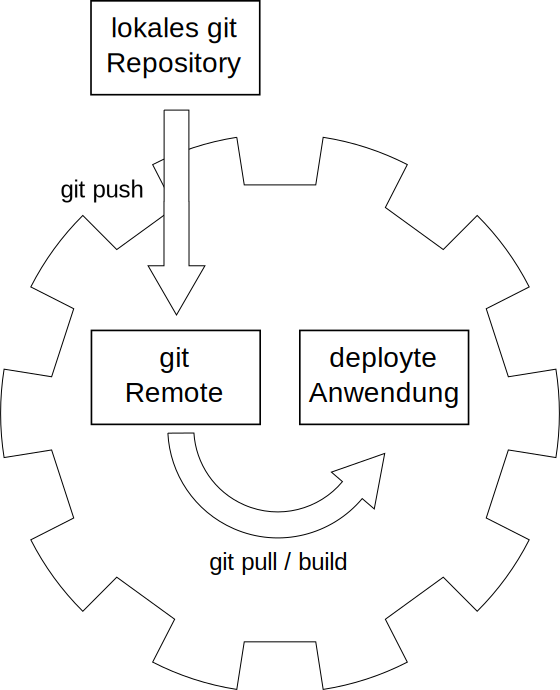
\includegraphics[width=0.7\linewidth]{imgs/deployment}
\caption{Ablauf des Deployments einer OpenShift Anwendung.}
\label{fig:deployment}
\end{figure}

Da das Beenden und Neustarten einer Anwendung beim Deployment längere Zeit dauern kann und somit störende Ausfallzeiten dieser bedeutet, unterstützt OpenShift für die meisten An\-wen\-dungs\-ser\-ver auch hot Deployment. Ist die Markerdatei \verb!.openshift/markers/hot_deploy! vorhanden, erfolgt das Deployment ohne Neustart der Anwendung \cite[S.40f]{os_user_guide}.

Große Anwendungen können teilweise aufgrund begrenzter Ressourcen oder zu starker Beeinträchtigung der laufenden Instanz nicht innerhalb des Anwendungsgears gebaut werden. OpenShift ermöglicht aus diesem Grund die Nutzung eines Jenkins-Buildservices, der in einem eigenen Gear läuft, bei jedem \verb!git push! die Anwendung neu baut, und das Deployment startet, sollte der Bau erfolgreich verlaufen sein.
Nach 15 Minuten Inaktivität wird der Buildservice wieder gestoppt und das Gear wieder freigegeben \cite[S.45]{os_user_guide}.

Um eine genaue Kontrolle über den Start, eventuelle Migration von Daten, das Anlegen der Datenbankschemata oder Aufräumarbeiten beim Beenden der Anwendung zu erhalten stehen mehrere Hooks zum Ausführen von Skripten bereit. Diese Skripte sind nicht auf bestimmte Sprachen festgelegt; es können neben compilierten Programmen auch fast alle gängigen Skriptsprachen wie bash, perl, lua, ruby und python verwendet werden. Eine Auflistung möglicher Hooks liefert Tabelle~\ref{tab:hooks}.

\begin{table}[htbp]
\centering
\begin{tabularx}{\columnwidth}{lX}
\toprule
Name des Skripts & Beschreibung \\
\midrule
pre\_build & Die alte Version der Anwendung wurde gestoppt, die neue Version wurde gepusht aber noch nicht gebaut. \\
build & Die Anwendung wurde gebaut, aber noch nicht deployed. \\
deploy & Die Anwendung wurde deployed aber noch nicht gestartet. \\
post\_deploy & Ausgeführt direkt nachdem die neue Version der Anwendung gestartet wurde. \\
\bottomrule
\end{tabularx}
\caption{Übersicht nutzbarer Hooks in OpenShift.}
\label{tab:hooks}
\end{table}

Zusätzlich bietet OpenShift auch einen direkten ssh-Zugriff auf die Anwendung an, sodass das testen kleinerer Konfigurationsänderungen, der Zugriff auf Logs und eventuelle Debuggingarbeiten schnell und ohne Änderungen an den Deploymentskripten erfolgen kann.

\subsection{Skalieren von Anwendungen/Limitierungen}
\label{sec:scale}
OpenShift führt Anwendungen in sogenannten Gears aus. Ein kleines Gear verfügt über 512~MB Arbeitsspeicher, sowie über 1~GB persistenten Speicher. Anwendungen können entweder in nur einem Gear laufen oder über mehrere Gears skaliert werden. Ob eine Anwendung skaliert muss beim Erstellen angegeben werden und lässt sich danach nicht mehr ändern. Eine skalierende Anwendung erhält dabei automatisch HAProxy als Cartridge zum Monitoring und load-Balancing. HAProxy belegt dabei immer ein eigenes Gear, sodass eine skalierende Anwendung immer mindestens zwei Gears belegt. Zusätzlich spielt die gewählte Plattform eine wichtige Rolle, ob sich eine Anwendung skalieren lässt. Grundsätzlich lassen sich Anwendungen die persistent Daten im Dateisystem speichern oder einen globalen Zustand besitzen nicht skalieren \cite[S.28]{os_user_guide}.

\begin{figure}[htbp]
\centering
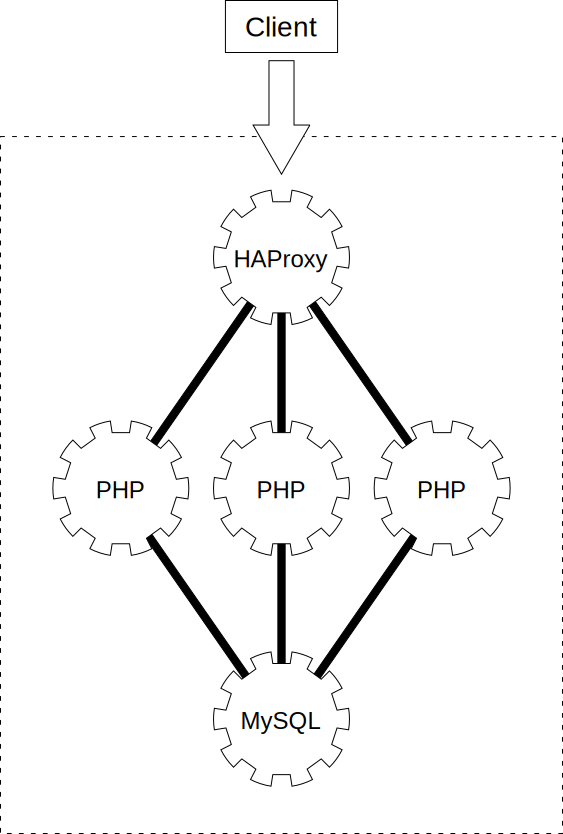
\includegraphics[width=0.8\linewidth]{imgs/scaling}
\caption{Aufbau einer skalierenden OpenShift Anwendung mit fünf Gears.}
\label{fig:scaling}
\end{figure}

Anwendungen lassen sich in zwei Richtungen skalieren: es können sowohl einzelne Cartridges in seperaten Gears laufen, als auch neue Anwendungsinstanzen erzeugt werden, sodass mehrere Gears Anfragen entgegen nehmen. Für eine optimale Verteilung der Anfragen wird dabei automatisch ein Load-Balancer vorgeschaltet. Falls ein Kunde über freie Gears verfügt, die der Anwendung bereitgestellt wurden und die Last einen Grenzwert von 90\% überschreitet wird automatisch eine neue Anwendungsinstanz erstellt und gestartet. Fällt die Last einer Instanz über längere Zeit wieder unter 50\%, werden die Gears wieder freigegeben \cite{os_scaling}. In Zukunft sollen sich diese Grenzwerte auch konfigurieren lassen um Kosten zu sparen oder die Leistung zu erhöhen. Derzeit lässt sich die automatische Skalierung nur beeinflussen, indem man die maximale und minimale Anzahl der zu nutzenden Gears beschränkt.

Eine weitere Limitierung besteht darin, dass OpenShift nur Verbindungen an Port 80 (HTTP), 443 (HTTPS) und 22 (SSH) akzeptiert. Zusätzlich werden nur HTTP/HTTPS durch den vorgeschalteten HTTP-Proxy weitergeleitet. Eine Nutzung anderer Protokolle ist deshalb nur durch Tunneling möglich.

\section{Technische Grundlagen}
\label{sec:tech}
Um die Skalierbarkeit und Verfügbarkeit der via OpenShift angebotenen Anwendungen zu gewährleisten sind bei der Implementierung von OpenShift selbst einige Probleme zu lösen: Die Plattform selbst muss leicht skalier- und erweiterbar sein und sich verteilt auch in weit entfernten Rechenzentren betreiben lassen um nicht selbst zum Flaschenhals für die Anwendungsperformance zu werden.

Da bei einem stark verteilten System die Aus\-fall\-wahr\-schein\-lich\-keit einzelner Knoten groß ist, darf der Betrieb der Plattform auch nicht durch den Ausfall einzelner Systeme beeinträchtigt werden; beziehungsweise müssen diese sich im Betrieb neu starten lassen und während dieser Zeit die Arbeit durch redundante Systeme übernommen werden.

\subsection{Anforderungen an Hosts}
OpenShift ist zur Nutzung mit RHEL ausgelegt, kann aber auch mit freien Klonen wie Scientific Linux oder CentOS sowie Fedora verwendet werden. Daher kann OpenShift Origin seinerseits populäre IaaS Dienste wie Amazon EC2 oder Openstack als Ausführungsumgebung nutzen. Des Weiteren nutzt OpenShift eine Vielzahl weiterer freier Projekte wie Bind, Apache ActiveMQ und MongoDB \cite[3.1]{os_buildyourown}.

\subsection{Allgemeine Architektur und Redundanz}
OpenShift besteht aus zwei verschiedenen Hosttypen: Nodes und Broker. Nodes dienen der Ausführung mehrerer Gears, Broker übernehmen die Steuerung und Management der Anwendungen. Zur internen Kommunikation zwischen Nodes und Broker wird das auf Apache ActiveMQ aufsetzende MCollective verwendet.
Bei der Implementierung sämtlicher Komponenten stand Redundanz im Vordergrund \cite[2.1]{os_buildyourown}, das heißt Broker können redundant verwendet werden, da sie zustandslos sind und auch MCollective kann mehrere ActiveMQ Instanzen verwenden. Da die Broker MongoDB als Datenbank nutzen, kann auch diese mittels Replica-Sets redundant verwendet werden. Abbildung~\ref{fig:architecture} verdeutlicht den Aufbau einer OpenShift Installation mit nur einem Broker und mehreren Nodes.

\begin{figure}[htbp]
\centering
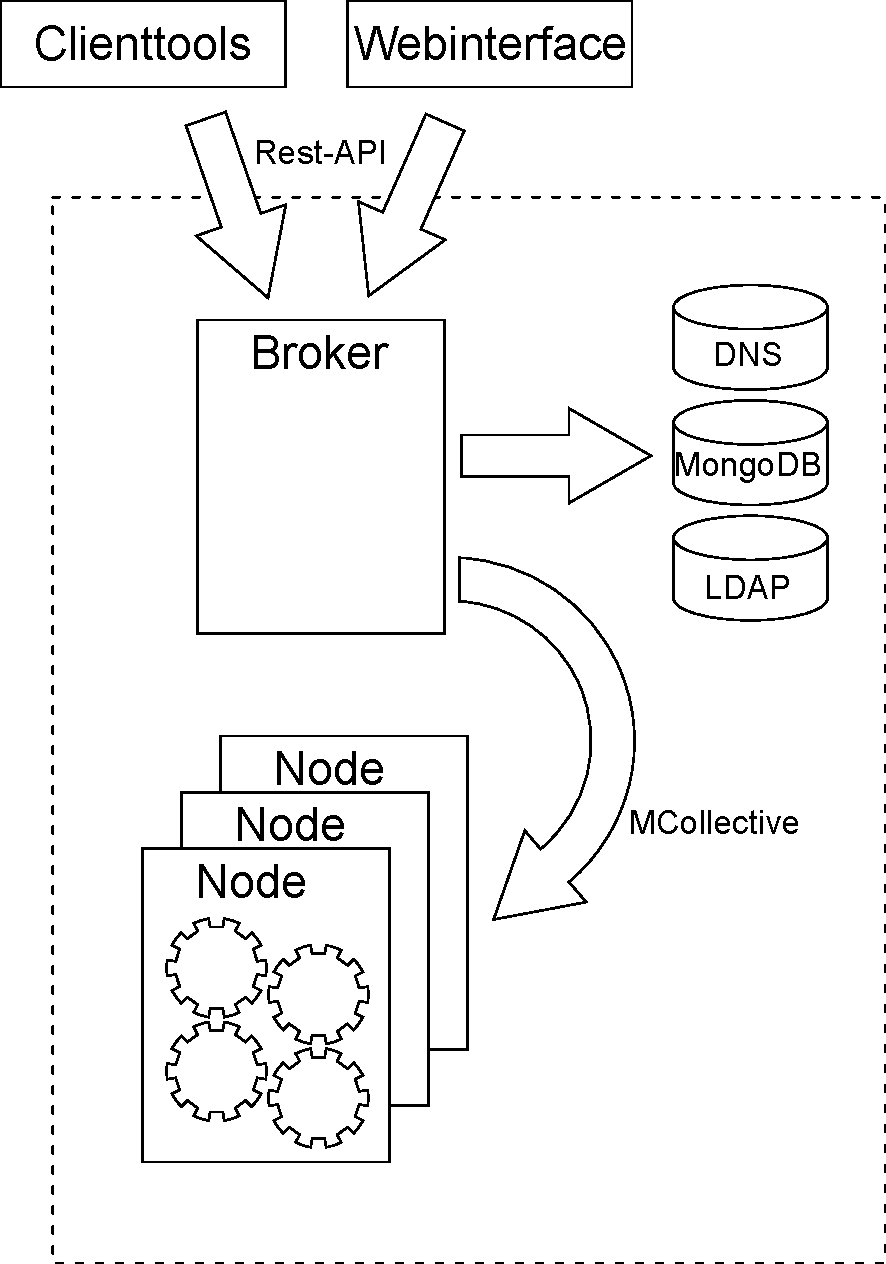
\includegraphics[width=0.8\linewidth]{imgs/architecture}
\caption{Schematischer Aufbau einer OpenShift Installation.}
\label{fig:architecture}
\end{figure}

\subsection{Nodes}
Die mittels OpenShift gehosteten Anwendungen laufen auf Nodes. Diese werden zur einfachen Verwaltung der Ressourcen in logische Gears aufgeteilt. Ein einzelner Node kann dabei eine Vielzahl Gears ausführen um eine möglichst hohe Auslastung zu erreichen. Zur fairen Nutzung gemeinsamer Ressourcen zwischen Gears nutzt OpenShift Linux Kernel cgroups, mit denen sich für Prozessgruppen CPU-Zeit, Arbeitsspeicher inklusive Dateisystemcaches und Netzwerkbandbreite limitieren lassen. Disk Quotas stellen zusätzlich sicher, dass ein Gear nicht zu viel Speicher belegt. Mittels SELinux werden zusätzlich enge Richtlinien gesetzt um Gears vollständig voneinander abzuschotten \cite[3.5]{os_buildyourown}. Zusammen sorgen all diese Maßnahmen dafür, dass auch ohne Ressourcenintensive Maßnahmen wie eine vollständige Virtualisierung mehrere Gears unabhängig auf einem Node laufen können.

\subsection{Broker}
Der zweite Hosttyp einer OpenShift installation sind Broker. Diese verwalten die Nodes, erzeugen Anwendungsinstanzen, allokieren weitere Gears bei zusätzlichem Ressourcenbedarf und geben diese wieder frei, falls kein weiterer Bedarf besteht oder die Anwendung gestoppt wird.

Des Weiteren kümmert sich der Broker um den kompletten Zustand der Anwendungen: DNS-Einträge werden durch Bind verwaltet, Benutzerauthentifizierung erfolgt durch LDAP oder Kerberos, der restliche Zustand in einer MongoDB gehalten.

Die Hauptarbeit übernimmt dabei eine auf dem Broker laufende Rails-Anwendung, die über eine Rest-API
angesprochen werden kann und andererseits via MCollective mit den Nodes kommunizieren kann.

Bei skalierbaren Anwendungen kann die jeweils laufende HAProxy Cartridge über den Broker mittels der Rest-API die Allokation weiterer Gears veranlassen falls dem Nutzer weitere Gears zur Verfügung stehen oder umgekehrt bei geringer Last dies an den Broker melden um eine Reduzierung der parallelen Instanzen zu erreichen.

\subsection{Rest API}
Der Broker selbst bietet keine direkte Nutzerschnittstelle, sondern nur eine Rest-API über die er sich ansprechen lässt \cite{os_rest}. Diese wird beispielsweise durch die Weboberfläche und die Clienttools implementiert.
Die Weboberfläche ist dabei eine einfache Webanwendung, die beispielsweise selbst wieder mittels OpenShift gehostet werden kann. Die Clienttools sind eine Sammlung in Ruby geschriebener Kommandozeilenprogramme, die die API menschenlesbar verfügbar machen.

Die OpenShift API hält sich an die „Hypermedia as the engine of application state“ (HATEOAS) Prinzip \cite{dis_rest}; das heißt nur ein einziger Zugangspunkt der API muss dem Client bekannt sein, weitere Zugangspunkte, Methoden und Parameter verschickt der Server daraufhin als Antwort an den Client.

Beispielhaft könnte das Erstellen einer neuen Anwendung in folgenden Schritten ablaufen:
Der Client sendet mittels Basic Authentication seinen Nutzernamen und Passwort an den API-Zugangspunkt \url{https://openshift.redhat.com/broker/rest/api}; die Antwort des Servers enthält unter anderem den Status, die unterstützten API-Versionen und weitere Zugangspunkte zur API.
Der Antwort kann der Link zum Erstellen einer neuen Nutzer-Domain entnommen werden; mittels Post wird der Name an \url{https://openshift.redhat.com/broker/rest/domains} gesendet.
Nun kann wieder mittels Post eine neue Anwendung erstellt werden: \url{https://openshift.redhat.com/broker/rest/domains/[Domain_ID]/applications}, wobei unter anderem der Anwendungsname und die Basis-Cartridge angegeben werden müssen.
Im letzten Schritt kann mittels Post noch ein Startevent an \url{https://openshift.redhat.com/broker/rest/domains/[Domain_ID]/applications/[App_Name]/events} gesendet werden um die Anwendung zu starten.

\subsection{Kommunikation}
Neben der Rest-API zur Kommunikation mit den Clienttools benötigt ein Broker eine Möglichkeit um mit den Nodes zu Kommunizieren. OpenShift nutzt Marionette Collective (MCollective) um einerseits Broadcasts an bestimmten Filterregeln entsprechenden, oder alle Nodes versenden zu können und andererseits einen RPC-Mechanismus zu implementieren um Anwendungen zu starten, stoppen, skalieren oder auf andere Nodes zu verlagern.

\subsection{DNS}
Zur Vergabe dynamischer Hostnames für die einzelnen Anwendungen vergibt OpenShift Subdomains nach dem Namensschema
[App\_Name]-[Suffix]. Suffix ist dabei ein vom Nutzer gewählter Namensraum, den alle Anwendungen eines Nutzers gemein haben. Zusätzlich kann vom Benutzer auch ein alias vergeben werden, falls die Anwendung unter anderem Domainnamen laufen soll.

Derzeit kann als DNS-Server einer OpenShift-Installation nur Bind verwendet werden; da das für DNS updates zuständige Plugin aber austauschbar ist, können theoretisch auch alternative DNS-Server verwendet werden, wenn ein entsprechendes Plugin dafür geschrieben wird \cite[3.4.2]{os_buildyourown}.

\section{Zusammenfassung}
\label{sec:sum}
OpenShift ist ein noch recht junges Projekt, das noch aktiv weiterentwickelt wird und sich ständig verändert. Dennoch bietet die Plattform schon heute eine große Zahl möglicher Anwendungsszenarien durch die Vielzahl unterstützter Anwendungsserver und Sprachen. Die Möglichkeit OpenShift nicht als durch Red Hat angebotenen Dienst zu nutzen, sondern auch selbst zu hosten gepaart mit dem streng auf Skalierbarkeit und Redundanz ausgelegten Design machen den Dienst sowohl für kleine Startups oder mittelständische Firmen mit wenigen eigenen Servern, als auch für Betreiber ganzer Rechenzentren interessant. In wie weit sich diese Offenheit gegen viel größere Wettbewerber mit starkem Vendor Lock-in durchsetzen kann lässt sich derzeit jedoch noch nicht absehen.

%\nocite{*}
\bibliographystyle{IEEEtranS}
\bibliography{references}

\end{document}
